%%%%%%%%%%%%%%%%%%%%%%%%%%%%%%%%%%%%%%%%%
% Adapted from
% Stylish Article
% LaTeX Template
% Version 1.0 (31/1/13)
%
% This template has been downloaded from:
% http://www.LaTeXTemplates.com
%
% Original author:
% Mathias Legrand (legrand.mathias@gmail.com)
%
% License:
% CC BY-NC-SA 3.0 (http://creativecommons.org/licenses/by-nc-sa/3.0/)
%
%%%%%%%%%%%%%%%%%%%%%%%%%%%%%%%%%%%%%%%%%


%----------------------------------------------------------------------------------------
%	PACKAGES AND OTHER DOCUMENT CONFIGURATIONS
%----------------------------------------------------------------------------------------

\documentclass[fleqn,10pt]{latex/stylish_article} % Document font size and equations flushed left

\setcounter{tocdepth}{3} % Show only three levels in the table of contents section: sections, subsections and subsubsections


% Pandoc environments
\usepackage{framed}
\usepackage{fancyvrb}
\providecommand{\tightlist}{%
  \setlength{\itemsep}{0pt}\setlength{\parskip}{0pt}}
\newcommand{\VerbBar}{|}
\newcommand{\VERB}{\Verb[commandchars=\\\{\}]}
\DefineVerbatimEnvironment{Highlighting}{Verbatim}{commandchars=\\\{\}, fontsize=\scriptsize} % Code R
\definecolor{shadecolor}{RGB}{248,248,248}
\newenvironment{Shaded}{\begin{snugshade}}{\end{snugshade}}
\newcommand{\KeywordTok}[1]{\textcolor[rgb]{0.13,0.29,0.53}{\textbf{{#1}}}}
\newcommand{\DataTypeTok}[1]{\textcolor[rgb]{0.13,0.29,0.53}{{#1}}}
\newcommand{\DecValTok}[1]{\textcolor[rgb]{0.00,0.00,0.81}{{#1}}}
\newcommand{\BaseNTok}[1]{\textcolor[rgb]{0.00,0.00,0.81}{{#1}}}
\newcommand{\FloatTok}[1]{\textcolor[rgb]{0.00,0.00,0.81}{{#1}}}
\newcommand{\ConstantTok}[1]{\textcolor[rgb]{0.00,0.00,0.00}{{#1}}}
\newcommand{\CharTok}[1]{\textcolor[rgb]{0.31,0.60,0.02}{{#1}}}
\newcommand{\SpecialCharTok}[1]{\textcolor[rgb]{0.00,0.00,0.00}{{#1}}}
\newcommand{\StringTok}[1]{\textcolor[rgb]{0.31,0.60,0.02}{{#1}}}
\newcommand{\VerbatimStringTok}[1]{\textcolor[rgb]{0.31,0.60,0.02}{{#1}}}
\newcommand{\SpecialStringTok}[1]{\textcolor[rgb]{0.31,0.60,0.02}{{#1}}}
\newcommand{\ImportTok}[1]{{#1}}
\newcommand{\CommentTok}[1]{\textcolor[rgb]{0.56,0.35,0.01}{\textit{{#1}}}}
\newcommand{\DocumentationTok}[1]{\textcolor[rgb]{0.56,0.35,0.01}{\textbf{\textit{{#1}}}}}
\newcommand{\AnnotationTok}[1]{\textcolor[rgb]{0.56,0.35,0.01}{\textbf{\textit{{#1}}}}}
\newcommand{\CommentVarTok}[1]{\textcolor[rgb]{0.56,0.35,0.01}{\textbf{\textit{{#1}}}}}
\newcommand{\OtherTok}[1]{\textcolor[rgb]{0.56,0.35,0.01}{{#1}}}
\newcommand{\FunctionTok}[1]{\textcolor[rgb]{0.00,0.00,0.00}{{#1}}}
\newcommand{\VariableTok}[1]{\textcolor[rgb]{0.00,0.00,0.00}{{#1}}}
\newcommand{\ControlFlowTok}[1]{\textcolor[rgb]{0.13,0.29,0.53}{\textbf{{#1}}}}
\newcommand{\OperatorTok}[1]{\textcolor[rgb]{0.81,0.36,0.00}{\textbf{{#1}}}}
\newcommand{\BuiltInTok}[1]{{#1}}
\newcommand{\ExtensionTok}[1]{{#1}}
\newcommand{\PreprocessorTok}[1]{\textcolor[rgb]{0.56,0.35,0.01}{\textit{{#1}}}}
\newcommand{\AttributeTok}[1]{\textcolor[rgb]{0.77,0.63,0.00}{{#1}}}
\newcommand{\RegionMarkerTok}[1]{{#1}}
\newcommand{\InformationTok}[1]{\textcolor[rgb]{0.56,0.35,0.01}{\textbf{\textit{{#1}}}}}
\newcommand{\WarningTok}[1]{\textcolor[rgb]{0.56,0.35,0.01}{\textbf{\textit{{#1}}}}}
\newcommand{\AlertTok}[1]{\textcolor[rgb]{0.94,0.16,0.16}{{#1}}}
\newcommand{\ErrorTok}[1]{\textcolor[rgb]{0.64,0.00,0.00}{\textbf{{#1}}}}
\newcommand{\NormalTok}[1]{{#1}}

% cslreferences environment required by pandoc > 2.7


% Tables
\usepackage{longtable,booktabs}
\usepackage{caption}
% These lines are needed to make table captions work with longtable:
\makeatletter
\def\fnum@table{\tablename~\thetable}
\makeatother
% longtable 2 columns
% https://tex.stackexchange.com/questions/161431/how-to-solve-longtable-is-not-in-1-column-mode-error
\makeatletter
\let\oldlt\longtable
\let\endoldlt\endlongtable
\def\longtable{\@ifnextchar[\longtable@i \longtable@ii}
\def\longtable@i[#1]{\begin{figure}[t]
\onecolumn
\begin{minipage}{0.5\textwidth}\scriptsize
\oldlt[#1]
}
\def\longtable@ii{\begin{figure}[t]
\onecolumn
\begin{minipage}{0.5\textwidth}\scriptsize
\oldlt
}
\def\endlongtable{\endoldlt
\end{minipage}
\twocolumn
\end{figure}}
\makeatother

% Figures
\usepackage{graphicx,grffile}
\makeatletter
\def\maxwidth{\ifdim\Gin@nat@width>\linewidth\linewidth\else\Gin@nat@width\fi}
\def\maxheight{\ifdim\Gin@nat@height>\textheight0.8\textheight\else\Gin@nat@height\fi}
\makeatother
% Scale images if necessary, so that they will not overflow the page
% margins by default, and it is still possible to overwrite the defaults
% using explicit options in \includegraphics[width, height, ...]{}
\setkeys{Gin}{width=\maxwidth,height=\maxheight,keepaspectratio}

% User-adder preamble
\usepackage{textcomp}

\DeclareUnicodeCharacter{B0}{\textdegree}

\usepackage{tabu} \renewenvironment{table}{\begin{table*}}{\end{table*}\ignorespacesafterend} \hyphenation{bio-di-ver-si-ty sap-lings}

%----------------------------------------------------------------------------------------
%	ARTICLE INFORMATION
%----------------------------------------------------------------------------------------

\JournalInfo{Publication reference} % Journal information
\Archive{DOI: xxx/xx} % Additional notes (e.g. copyright, DOI, review/research article)

\PaperTitle{Title of the Article} % Article title

\Authors{
First Author's name\textsuperscript{1*}\\ Second Author's name\textsuperscript{2}
} % Authors
\affiliation{
\textsuperscript{1}Department / University\\ \hspace{1em} Street address, Zip code, Country.\\\textsuperscript{2}Department / University\\ \hspace{1em} Street address, Zip code, Country.
}
\affiliation{*\textbf{Corresponding author}: \href{mailto:name@company.com}{\nolinkurl{name@company.com}}, \url{https://www.company.com}} % Corresponding author

\Keywords{keyword1, keyword2, etc} % Keywords - if you don't want any simply remove all the text between the curly brackets
\newcommand{\keywordname}{Keywords} % Defines the keywords heading name

%----------------------------------------------------------------------------------------
%	ABSTRACT
%----------------------------------------------------------------------------------------

\Abstract{
Summary of the article.
}

%----------------------------------------------------------------------------------------

\begin{document}

\selectlanguage{english}

\flushbottom % Makes all text pages the same height

\maketitle % Print the title and abstract box

\tableofcontents % Print the contents section

\thispagestyle{empty} % Removes page numbering from the first page

%----------------------------------------------------------------------------------------
%	ARTICLE CONTENTS
%----------------------------------------------------------------------------------------


\hypertarget{introduction}{%
\section{Introduction}\label{introduction}}

Ce modèle permet la rédaction d'articles au format Markdown\footnote{\url{https://ericmarcon.github.io/travailleR/chap-rediger.html}}.
Il produit directement des articles bien formatés pour l'auto-archivage (dépôt sur HAL par exemple) ou sous d'autres formats, par exemple HTML.

\hypertarget{markdown}{%
\section{R Markdown}\label{markdown}}

Markdown est un langage très simple pour produire divers types de documents: HTML, PDF, et Word entre autres.
Sa documentation est disponible sur le site de RStudio\footnote{\url{http://rmarkdown.rstudio.com/articles.html}}.

Markdown est étendu par Bookdown\footnote{\url{https://bookdown.org/yihui/bookdown/}}, qui permet la rédaction de livres et une syntaxe plus efficace pour les articles.
Ce document est réalisé avec Markdown dans RStudio: knitr traite le code Markdown, le passe à Pandoc pour sa transformation en LaTeX, enfin LateX le compile en PDF.

\hypertarget{intuxe9ruxeat}{%
\subsection{Intérêt}\label{intuxe9ruxeat}}

Markdown est très simple à apprendre.

Markdown permet d'intégrer son code R pour un résultat \emph{reproductible}.

Markdown permet de produire, sans réécrire le texte, un document dans différents formats: article LaTeX ou Word par exemple.

\hypertarget{comment-faire}{%
\subsection{Comment faire}\label{comment-faire}}

Dans RStudio, créer un nouveau document de type Document R Markdown.
L'assistant permet de choisir entre divers formats.

\scriptsize

\begin{figure}

{\centering 
\includegraphics[width=0.8\linewidth]{images/logo} 

}

\caption{Nouveau document}\label{fig:nouveau}
\end{figure}

\normalsize

Cliquer sur \emph{From template}: à partir de modèles installés par des packages.
Les modèles du package EcoFoG sont affichés (voir figure \ref{fig:nouveau}): choisir Article EcoFoG.

Ecrire le document dans RStudio.

Cliquer sur le bouton \textbf{Knit} de RStudio génère le document au format demandé.

Il est préférable de créer un projet RStudio pour bénéficier de toutes les possiblités : \emph{File} / \emph{New Project} puis utiliser l'assistant pour créer un projet à partir d'un dossier existant.

\hypertarget{code}{%
\section{Code}\label{code}}

Les principales caractéristiques de Markdown sont résumées ici.

\hypertarget{code-r}{%
\subsection{Code R}\label{code-r}}

Le code R est inclus dans des bouts de code (\emph{code chunks}):

\scriptsize

\begin{Shaded}
\begin{Highlighting}[]
\KeywordTok{head}\NormalTok{(cars)}
\end{Highlighting}
\end{Shaded}

\begin{verbatim}
##   speed dist
## 1     4    2
## 2     4   10
## 3     7    4
## 4     7   22
## 5     8   16
## 6     9   10
\end{verbatim}

\normalsize

\hypertarget{tableaux}{%
\subsection{Tableaux}\label{tableaux}}

Les séparateurs horizontaux - et verticaux \textbar{} permettent de dessiner un tableau selon la syntaxe de Markdown, mais ce n'est pas la meilleure méthode.

Les tableaux peuvent aussi être produits par du code R.
Le contenu du tableau est dans un dataframe.
La fonction \texttt{kable} du package \emph{knitr} prépare le tableau pour l'affichage et passe le résultat à la fonction \texttt{kable\_styling} du package \emph{kableExtra} pour le formatage final.

\scriptsize

\begin{longtable}[t]{rrrrl}
\caption{\label{tab:kable}Tableau créé par R}\\
\toprule
Longueur sépales & Largeur & Longueur pétales & Largeur & Espèce\\
\midrule
5.1 & 3.5 & 1.4 & 0.2 & setosa\\
4.9 & 3.0 & 1.4 & 0.2 & setosa\\
4.7 & 3.2 & 1.3 & 0.2 & setosa\\
4.6 & 3.1 & 1.5 & 0.2 & setosa\\
5.0 & 3.6 & 1.4 & 0.2 & setosa\\
\addlinespace
5.4 & 3.9 & 1.7 & 0.4 & setosa\\
\bottomrule
\end{longtable}

\normalsize

La légende est précisée par l'argument \texttt{caption} et le référencement est possible parce que le tableau reçoit une étiquette dont le nom est \texttt{tab:} suivi du nom du bout de code (tableau \ref{tab:kable}).
Utiliser systématiquement l'argument \texttt{booktabs\ =\ TRUE} pour que l'épaisseur des lignes de séparation soit optimale en LaTeX.
L'option\break \texttt{bootstrap\_options\ =\ "striped"} fournit des tableaux plus lisibles en HTML.

En LaTeX, Les tableaux peuvent avoir la largeur de la colonne et éventuellement d'étendre sur plusieurs pages\break \texttt{longtable\ =\ TRUE} ou bien utliser la largeur de la page\break \texttt{longtable\ =\ FALSE} comme le tableau \ref{tab:Paracou}).

\scriptsize

\begin{table*}

\caption{\label{tab:Paracou}Intervention table, summary of the disturbance intensity for the 4 plot treatments in Paracou.}
\centering
\begin{tabu} to \linewidth {>{\raggedright}X>{\raggedright}X>{\raggedright}X>{\raggedright}X>{\raggedright}X}
\toprule
Treatment & Timber & Thinning & Fuelwood & \%AGB lost\\
\midrule
Control &  &  &  & 0\\
T1 & DBH $\geq$ 50 cm, commercial species, $\approx$ 10 trees/ha &  &  & $[12\%-33\%]$\\
T2 & DBH $\geq$ 50 cm, commercial species, $\approx$ 10 trees/ha & DBH $\geq$ 40 cm, non-valuable species, $\approx$ 30 trees/ha &  & $[33\%-56\%]$\\
T3 & DBH $\geq$ 50 cm, commercial species, $\approx$ 10 trees/ha & DBH $\geq$ 50 cm, non-valuable species, $\approx$ 15 trees/ha & 40 cm $\leq$ DBH $\leq$ 50 cm, non-valuable species, $\approx$ 15 trees/ha & $[35\%-56\%]$\\
\bottomrule
\end{tabu}
\end{table*}\ignorespacesafterend

\normalsize

Ce tableau contient des mathématiques : l'option\break \texttt{escape\ =\ FALSE} est nécessaire.

Enfin, l'option \texttt{full\_width\ =\ FALSE} permet d'ajuster la largeur du tableau à son contenu au lieu d'occuper toute la largeur disponible.
Elle doit être \texttt{TRUE} pour le formatage correct des tableaux sur deux colonnes en LaTeX.
Un bug de knitr fait que le format du tableau (``html'') n'est pas transmis correctement à \texttt{kable\_styling} lors du tricotage au format gitbook, ce qui génère un avertissement et empêche l'option d'être prise en compte.

\hypertarget{figures}{%
\subsection{Figures}\label{figures}}

\scriptsize

\begin{Shaded}
\begin{Highlighting}[]
\KeywordTok{plot}\NormalTok{(pressure)}
\end{Highlighting}
\end{Shaded}

\begin{figure}

{\centering 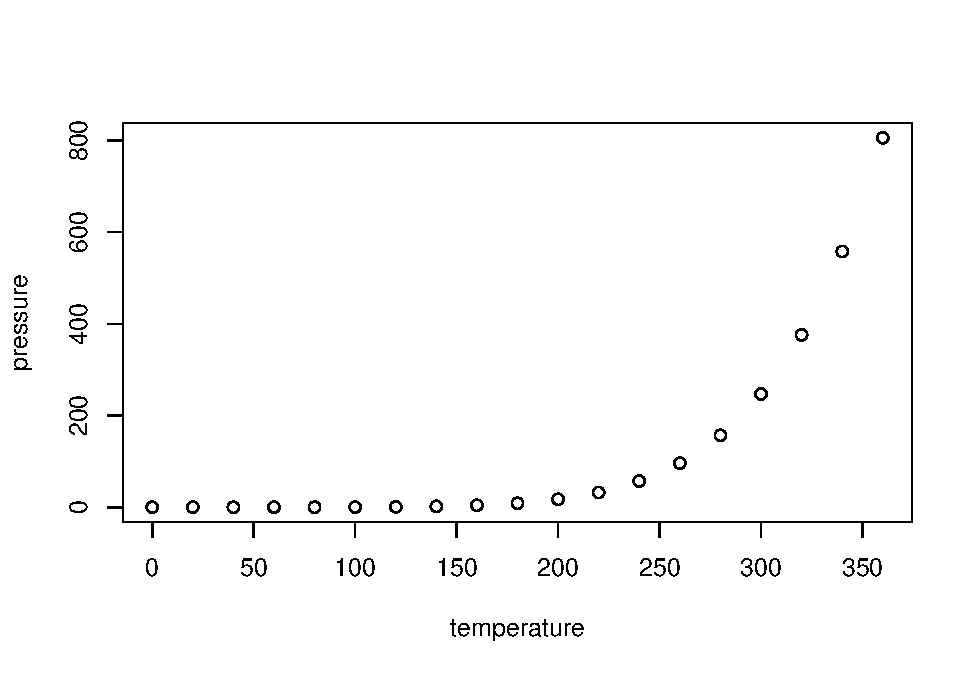
\includegraphics[width=0.8\linewidth]{/private/var/folders/24/8k48jl6d249_n_qfxwsl6xvm0000gn/T/RtmpllMaSh/stylish_article/gallery/stylish_article/stylish_article_files/figure-latex/pressure-1} 

}

\caption{Titre de la figure}\label{fig:pressure}
\end{figure}

\normalsize

Les figures peuvent être créées par le code R (figure \ref{fig:pressure}).
Avec Bookdown, une étiquette est associée à chaque figure: son nom est \texttt{fig:xxx} où \texttt{xxx} est le nom du bout de code R.
Les renvois se fonct avec la commande \texttt{\textbackslash{}@ref(fig:xxx)}.

Une figure peut utiliser toute la largeur de la page en ajoutant les options suivantes dans l'entête du bout de code qui la génère: \texttt{fig.env="figure*"} et\break \texttt{out.extra=""}.

Les figures existantes sont intégrées dans un bout de code par la fonction \texttt{include\_graphics}, voir la figure \ref{fig:nouveau}.
Placer systématiquement ces fichiers dans le dossier \texttt{images} pour l'automatisation des pages GitHub.

\hypertarget{listes}{%
\subsection{Listes}\label{listes}}

Les listes sont indiquées par des *, + et - (trois niveaux hiérarchiques) ou des nombres 1., i. et A. (listes numérotées).

\begin{itemize}
\tightlist
\item
  Liste

  \begin{itemize}
  \tightlist
  \item
    sous-liste
  \end{itemize}
\item
  deuxième élément
\item
  Suite de la liste
\end{itemize}

\hypertarget{maths}{%
\subsection{Maths}\label{maths}}

Les équations au format LaTeX peuvent être insérées en ligne, comme \(A=\pi r^2\) ou isolées comme \[e^{i \pi} = -1.\]

Elles peuvent être numérotées, voir équation \eqref{eq:disque}, en utilisant l'environnement \texttt{\textbackslash{}equation}:

\begin{equation}
A = \pi r^2.
\label{eq:disque}
\end{equation}

\hypertarget{ruxe9fuxe9rences-croisuxe9es}{%
\subsection{Références croisées}\label{ruxe9fuxe9rences-croisuxe9es}}

Les figures et tableaux ont une étiquette générée automatiquement, identique au nom du bout de code préfixé par \texttt{fig:} et \texttt{tab:}.

Pour les équations, l'étiquette est ajoutée manuellement par le code \texttt{(\textbackslash{}\#eq:xxx)} avant la fin de l'équation.

Les sections peuvent recevoir une étiquette en terminant leur titre par \texttt{\{\#yyy\}}.

Des signets peuvent aussi être placés librement dans le texte avec la commande \texttt{(ref:zzz)}.

Dans tous les cas, l'appel à la référence est fait par la commande \texttt{\textbackslash{}@ref(ref:zzz)}.

\hypertarget{bibliographie}{%
\subsection{Bibliographie}\label{bibliographie}}

Les références bibliographiques incluses dans le fichier references.bib peuvent être appelées dans le texte, entre parenthèses \citep{Xie2016}, ou dans le texte, à la façon de \citet{Xie2016}.

La bibliographie est traitée par Pandoc lors de la production de documents Word ou HTML.
Le style bibliographique peut être précisé, en ajoutant la ligne

\begin{verbatim}
csl:nom_du_fichier.csl
\end{verbatim}

dans l'entête du document et en copiant le fichier de style \emph{.csl} dans le dossier du projet.
Plus d'un millier de styles sont disponibles\footnote{\url{https://github.com/citation-style-language/styles}}.

Pour les documents PDF, la bibliographie est gérée par LaTeX.
Le style est inclus dans le modèle EcoFoG: c'est celui de \emph{Methods in Ecology and Evolution}.
Il ne peut pas être changé, pour assurer l'homogénéité des documents produits.

Pour préparer la soumission d'un manuscrit à une revue, il faudra ouvrir le fichier \emph{.tex} intermédiaire produit par Pandoc et copier le contenu de l'environnement \{document\} dans le modèle proposé par la revue, qui se chargera du formatage.

\hypertarget{pruxe9ambule-latex}{%
\subsection{Préambule LaTeX}\label{pruxe9ambule-latex}}

Des commandes LaTeX peuvent être ajoutées dans le préambule du fichier LaTeX produit, par exemple pour charger des packages supplémentaires.
Ces commandes sont dans la section \texttt{preamble:} de l'entête du fichier Markdown.

Les commandes par défaut permettent :

\begin{itemize}
\tightlist
\item
  d'utiliser le caractère degré (exemple: 20°C) :
\end{itemize}

\begin{verbatim}
\usepackage{textcomp}
\DeclareUnicodeCharacter{B0}{\textdegree}
\end{verbatim}

\begin{itemize}
\tightlist
\item
  d'obtenir des tableaux sur deux colonnes en redéfinissant l'environnement \texttt{table} et de charger le package \emph{tabu} nécessaire à \emph{kableExtra}:
\end{itemize}

\begin{verbatim}
\usepackage{tabu}
\renewenvironment{table}{%
  \begin{table*}}%
  {\end{table*}%
  \ignorespacesafterend
}
\end{verbatim}

\begin{itemize}
\tightlist
\item
  de montrer l'utilisation de la commande de césure:
\end{itemize}

\begin{verbatim}
\hyphenation%
  {bio-di-ver-si-ty sap-lings}
\end{verbatim}

D'autres commandes peuvent être ajoutées selon les besoins.
Attention :

\begin{itemize}
\tightlist
\item
  les commentaires ne sont pas possibles ;
\item
  les commandes complexes (comme\break \texttt{\textbackslash{}renewenvironment}) doivent être entrées sur une seule ligne sinon elles seront détruites par knitr au premier tricotage en HTML.
\end{itemize}

\hypertarget{foruxe7age-des-coupures-de-ligne}{%
\subsection{Forçage des coupures de ligne}\label{foruxe7age-des-coupures-de-ligne}}

La césure est gérée automatiquement en LaTeX.
Si un mot n'est pas coupé correctement, ajouter son découpage dans le préambule du fichier avec la commande \texttt{\textbackslash{}hyphenation} (les mots sont séparés par des espaces, les emplacement de césure représentés par des tirets).

Si LaTeX ne parvient pas à trouver de solution pour le retout à la ligne, par exemple pare que du code constitue un bloc insécable trop long, ajouter la commande LaTeX \texttt{\textbackslash{}break} à l'emplacement du retour à la ligne.
Ne pas laisser d'espace avant la commande.
Le document HTML ignore les commandes LaTeX.

\hypertarget{langues}{%
\subsection{Langues}\label{langues}}

L'Anglais et le Français sont supportés, à déclarer dans l'entête du document.

La langue choisie n'a d'effet que dans les sorties LaTeX: un espace est ajouté devant les ponctuations doubles en Français, la taille des espaces est plus grande en début de phrase en Anglais, etc.

Les modèles EcoFoG utilisent le package LaTeX \emph{babel} qui reconnaît les noms de langue \emph{french} et \emph{english}.
Pandoc utilise en revanche les codes IETF \emph{fr-FR} ou \emph{en-US} pour un support linguistique limité en HTML.
Les deux paramètres doivent donc être saisis dans l'entête du document.

\hypertarget{types-de-document}{%
\section{Types de document}\label{types-de-document}}

Ce modèle est prévu pour fonctionner avec le modèle Article d'EcoFoG en LaTeX et produire des documents au format PDF, HTML ou Word.
Utiliser la liste de choix du bouton \emph{Knit} pour choisir le format de sortie.

Le document Word peut ensuite être modifié pour respecter les instructions aux auteurs des revues : double interlignage, police, etc.

\hypertarget{document-pdf}{%
\subsection{Document PDF}\label{document-pdf}}

Le document est formaté pour l'auto-archivage d'articles bien mis en page.

\hypertarget{document-html}{%
\subsection{Document HTML}\label{document-html}}

Le modèle GitBook est optimisé pour la lecture sur écran.
Pendant toute l'écriture, préférer le tricot au format HTML pour sa vitesse d'exécution.
Un bouton de téléchargement est disponible dans la barre de menu du document: il fonctionnera si le document est aussi tricoté au format PDF et si le nom du fichier est rensigné dans le champ download de l'entête YAML.

Le modèle HMTL Book est une alternative.

\hypertarget{document-word}{%
\subsection{Document Word}\label{document-word}}

Son contenu peut être mis en forme ou copié dans un modèle.
Les styles de texte standard sont ``First Paragraph'' et ``Corps de de texte''.

L'intérêt du format Word est de produire un manuscrit pour les revues qui ne supportent pas LaTeX.
Le style bibliographique de la revue est très probablement disponible au format \emph{.csl}, ce qui permet de minimiser la préparation manuelle.

\hypertarget{optimisation-pour-github}{%
\subsection{Optimisation pour GitHub}\label{optimisation-pour-github}}

Le projet d'article peut être déposé sur Github\footnote{\url{https://ericmarcon.github.io/travailleR/chap-git.html}}.

Le script R fourni, \emph{GithubPages.R}, permet de publier facilement l'article dans les pages web associées au dépôt en déplaçant les fichiers HTML produit par le tricotage de l'article dans le dossier \emph{docs}.

Il suffit ensuite d'activer les pages web du dépôt, d'adapter le fichier \emph{README.md} fourni (suivre ses instructions) et de le dupliquer dans le dossier \emph{docs}.

Les pages web peuvent être produites par intégration continue\footnote{\url{https://ericmarcon.github.io/travailleR/chap-ci.html}}.

\hypertarget{autres-moduxe8les}{%
\subsection{Autres Modèles}\label{autres-moduxe8les}}

Le modèle de mémo EcoFoG est plus simple, formaté sur une seule colonne.

Le package \emph{rticle} fournit des modèles d'articles (PLOS, PNAS, etc.), mais nécessite l'utlisation de commandes LaTeX et ne permet pas le tricot en HTML.
Le package \emph{xaringan} fournit un modèle de présentation HTML 5.

Le modèle \emph{Ouvrage} du package EcoFoG permet d'écrire des livres.

La dernière ligne du modèle (bout de code R) doit être conservée pour afficher le titre \emph{References} (à traduire éventuellement dans la langue du document) au format HTML.
Le titre de niveau 1 \emph{Références} doit être ajouté manuellement aux fichiers Word.

%----------------------------------------------------------------------------------------
%	REFERENCE LIST
%----------------------------------------------------------------------------------------

\bibliographystyle{mee}
\makeatletter
% The filename has .bib extension that must be eliminated
\filename@parse{references.bib}
% parse stores the file name in base. Extension starts at the first dot, so don't use dots in file names.
\bibliography{\filename@base}
\makeatother


%----------------------------------------------------------------------------------------

\end{document}
